\documentclass[english,11pt]{beamer}

\DeclareMathOperator{\Cov}{Cov}
\DeclareMathOperator{\Var}{Var}
\DeclareMathOperator{\E}{\mathbb{E}}
\DeclareMathOperator{\Proba}{\mathbb{P}}

\newcommand{\Covb}[2]{\ensuremath{\Cov\!\left[#1,#2\right]}}
\newcommand{\Eb}[1]{\ensuremath{\E\!\left[#1\right]}}
\newcommand{\Pb}[1]{\ensuremath{\Proba\!\left[#1\right]}}
\newcommand{\Varb}[1]{\ensuremath{\Var\!\left[#1\right]}}

% norm
\newcommand{\norm}[1]{\| #1 \|}

\newcommand{\indep}{\rotatebox[origin=c]{90}{$\models$}}





\usepackage{mathptmx,amsmath,amssymb,graphicx,bibentry,bbm,babel,ragged2e}

\makeatletter

\newcommand{\noun}[1]{\textsc{#1}}
\newcommand{\jitem}[1]{\item \begin{justify} #1 \end{justify} \vfill{}}
\newcommand{\sframe}[2]{\frame{\frametitle{#1} #2}}

\newenvironment{centercolumns}{\begin{columns}[c]}{\end{columns}}
%\newenvironment{jitem}{\begin{justify}\begin{itemize}}{\end{itemize}\end{justify}}

\usetheme{Warsaw}
\setbeamertemplate{footline}[text line]{}
\setbeamercolor{structure}{fg=purple!50!blue, bg=purple!50!blue}

\setbeamersize{text margin left=15pt,text margin right=15pt}

\setbeamercovered{transparent}


\@ifundefined{showcaptionsetup}{}{%
 \PassOptionsToPackage{caption=false}{subfig}}
\usepackage{subfig}

\usepackage[utf8]{inputenc}
\usepackage[T1]{fontenc}



\makeatother

\begin{document}


\title{Investigating the Empirical Existence of Static User Equilibrium}

\author{J.~Raimbault$^{1,2}$\\
\texttt{juste.raimbault@parisgeo.cnrs.fr}
}


\institute{$^{1}$UMR CNRS 8504 G{\'e}ographie-cit{\'e}s\\
$^{2}$UMR-T IFSTTAR 9403 LVMT\\
}


\date{EWGT 2016 - Istanbul\\\smallskip
\textit{Session Transportation Modeling - MoST2-B}\\\smallskip5th September 2016
}

\frame{\maketitle}



%%%%%%%%%%%%%%%%%
\section{Introduction}
%%%%%%%%%%%%%%%%%



\sframe{Traffic Modeling : User Equilibrium Frameworks}{

\justify

% from static user eq to recent theoretical framework

\textit{Equilibrium frameworks central in Transportation Research since Wardrop \cite{wardrop1952road}}

\bigskip

\textbf{Diverse developments :}

\medskip

$\rightarrow$ Dynamic Stochastic User Equilibrium~\cite{han2003dynamic}

\medskip

$\rightarrow$ Restricted Stochastic User Equilibrium~\cite{rasmussen2015stochastic} more realistic in alternatives

\medskip

$\rightarrow$ Boundedly User Equilibrium~\cite{mahmassani1987boundedly}

\medskip

$\rightarrow$ Assignment techniques inspired from other fields such as Network Science~\cite{puzis2013augmented}

}


\sframe{Validation and Practical Use}{

\justify
% 

\textit{Static User Equilibrium lacks empirical validation in the literature}

\medskip

$\rightarrow$ Some examples such as the behavioral study of user route choices (``Wardrop's first principle'') in \cite{zhu2010people}

\bigskip


\textbf{However still largely used}

\medskip

$\rightarrow$ in theoretical literature, as for example \cite{leurent2014user} : do refinements in the model such as adding parking cruising flows have a sense if the core is not validated ?

\medskip

$\rightarrow$ in real-world application, such as the MODUS model for Paris Metropolitan area : what are the implications of basing decision-making and traffic management on an unvalidated framework ?


}


\sframe{Empirical Investigation of SUE Existence}{

\justify

\textbf{Research Objective : } \textit{Investigate empirically the spatio-temporal stationarity of traffic flows, combining different complementary quantitative approaches}

\bigskip

$\rightarrow$ Construction of a real-time dataset for major links of Paris region on 6 month by data crawling

\medskip

$\rightarrow$ Complementarity of approaches (Complex Systems general paradigm) : Spatio-temporal data visualization, Network analysis, Spatial analysis

}


%%%%%%%%%%%%%%%%%
\section{Methods and Results}
%%%%%%%%%%%%%%%%%



\sframe{Dataset Construction}{

\textit{Difficulty to find Open Data on Transportation Systems \cite{bouteiller2013open}}


$\rightarrow$ Construction of an open historical travel time dataset for major links in the region of Paris, collecting in real time public traffic data from \texttt{www.sytadin.fr}

\medskip

\textbf{Data collection : } Each two minutes, automated python script

\begin{itemize}
\item fetch raw webpage giving traffic information
\item parse html code
\item store in a \texttt{sqlite} database
\end{itemize}

\textit{Openly available (CC Licence) at }\texttt{\texttt{http://37.187.242.99/files/public/sytadin{\_}latest.sqlite3}}

\medskip

\textbf{Data summary : } 10 month (since Feb. 2016), 2min time granularity, effective travel time for 101 links ($\simeq$ 10km spatial granularity)


}



\sframe{Interactive Data Visualization}{

\textit{Interactive web-application for spatio-temporal exploration}

\texttt{http://shiny.parisgeo.cnrs.fr/transportation}

\bigskip

\centering


\includegraphics[width=0.9\textwidth]{figures/gr1}

}



\sframe{Spatio-temporal Variability : Example}{

\textit{Very high spatial variability on 10min time interval, here on 11/02/2016 00:06-00:16}

\bigskip

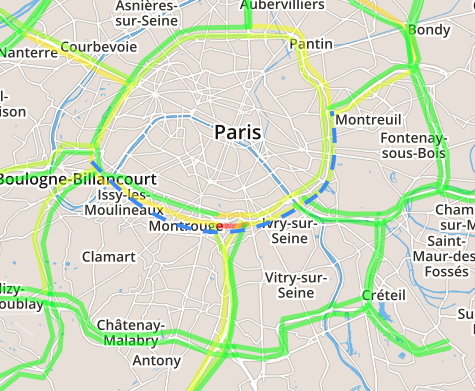
\includegraphics[width=0.48\textwidth]{figures/gr21}\hfill
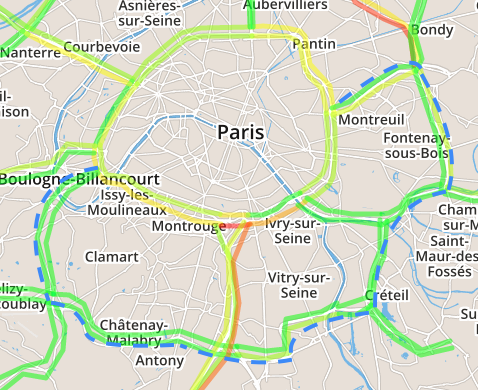
\includegraphics[width=0.48\textwidth]{figures/gr22}

}


\sframe{Spatio-temporal Variability}{

\textit{Maximal travel time and spatial variabilities on a two week sample}

\bigskip

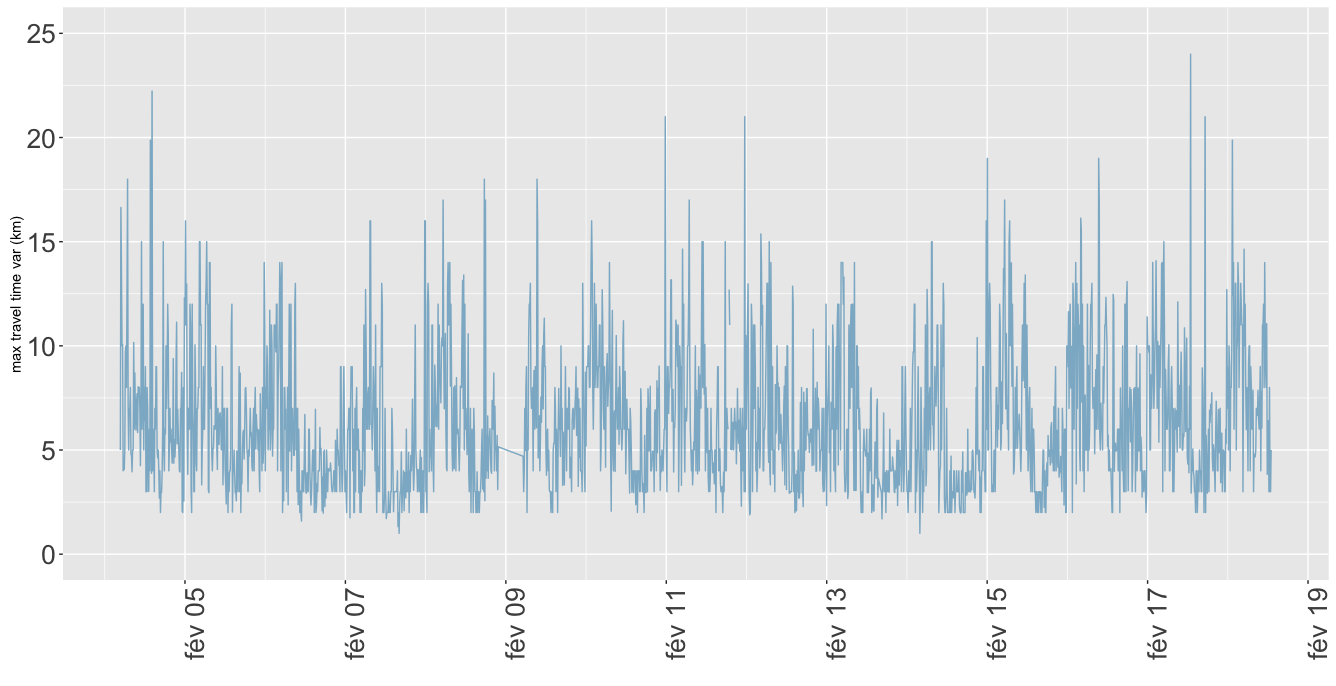
\includegraphics[width=0.5\textwidth,height=0.6\textheight]{figures/gr31}
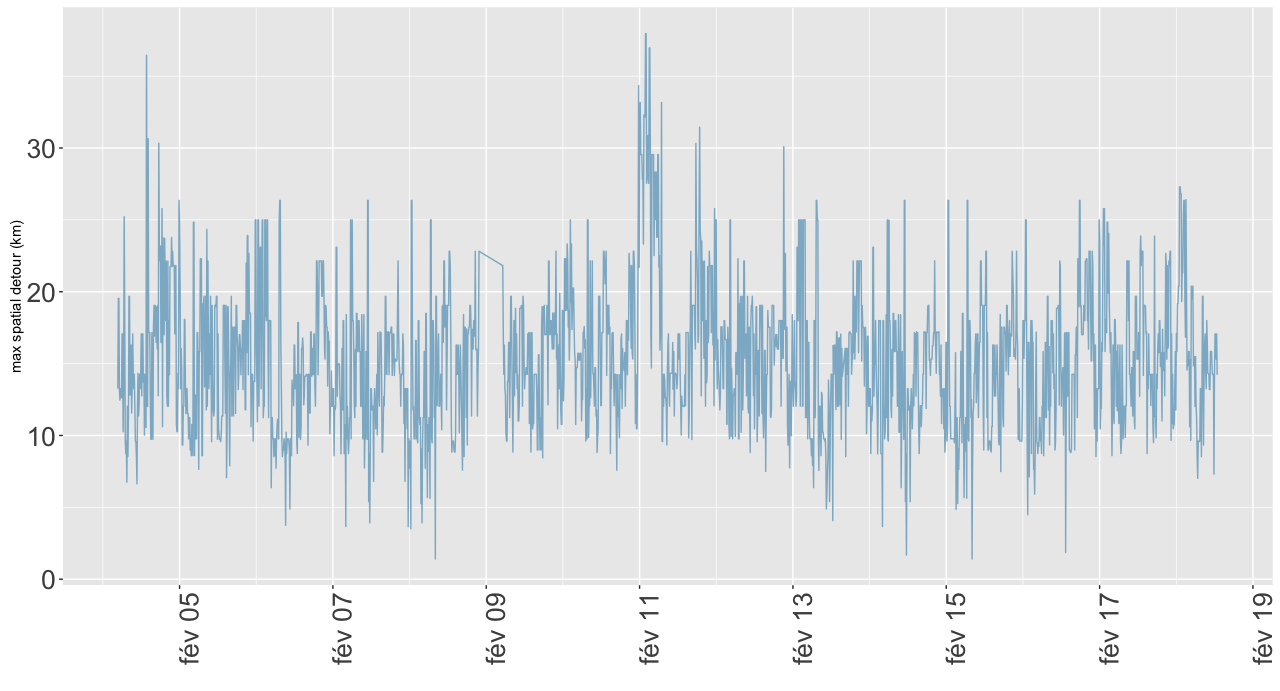
\includegraphics[width=0.5\textwidth,height=0.6\textheight]{figures/gr32}

}



\sframe{Stability of Network Measures}{

Network Betweenness Centrality 

\begin{equation}
b_i = \frac{1}{N(N-1)}\cdot \sum_{o\neq d \in V}\mathbbm{1}_{i\in p(o\rightarrow d)}
\end{equation}

Temporal Maximal Betweenness Variability

\begin{equation}
\Delta b(t) = \frac{\left|\max_i (b_i(t + \Delta t)) - \max_i (b_i(t))\right|}{\max_i (b_i(t))}
\end{equation}

\bigskip

$\rightarrow$ \textit{Reveals either a proportion of rerouted travels (negative variation) or a minimal proportion of load increase for a single node (positive variation)}

}


\sframe{Stability of Network Measures}{

\textit{Temporal maximal betweenness variability on a two weeks period}

\medskip

\centering 

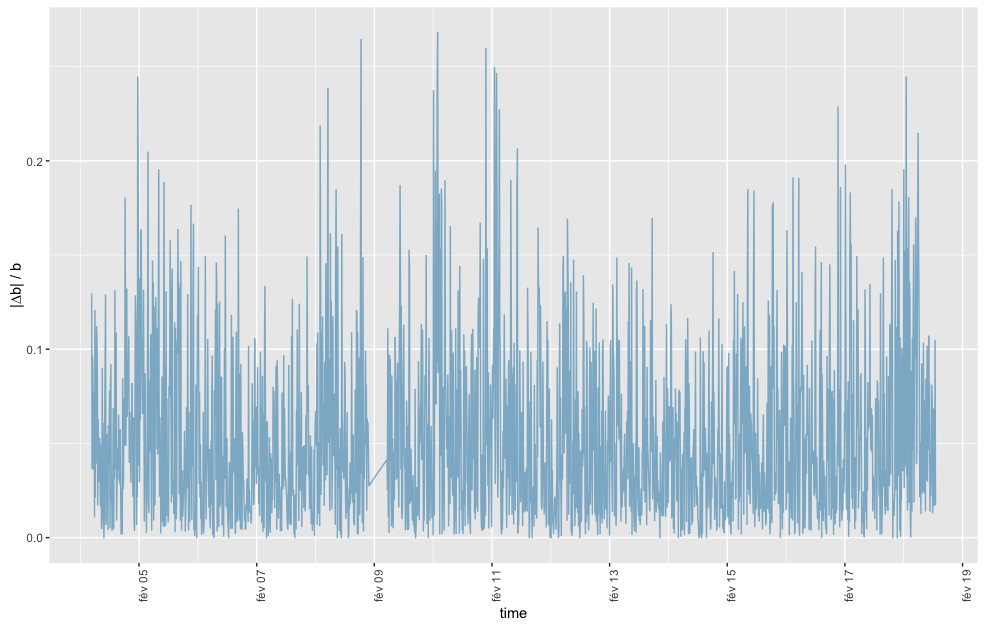
\includegraphics[width=0.9\textwidth]{figures/gr4}
}



\sframe{Spatial Heterogeneity}{

Spatial Autocorrelation as an index of spatial variability, for link $i$

\begin{equation}
\rho_i = \frac{1}{K}\cdot \sum_{i\neq j}{w_{ij}\cdot (c_i - \bar{c})(c_j - \bar{c})}
\end{equation}

with spatial weights  $w_{ij} = \exp{\left(\frac{-d_{ij}}{d_0}\right)}$

\bigskip
\bigskip

$\rightarrow$ \textit{Indirect measure of the spatial stationarity of flows : a decreasing correlation implies a chaotic system}


}



\sframe{Spatial Heterogeneity}{

\textit{Spatial autocorrelation on a two weeks period for different decays}

\medskip

\centering

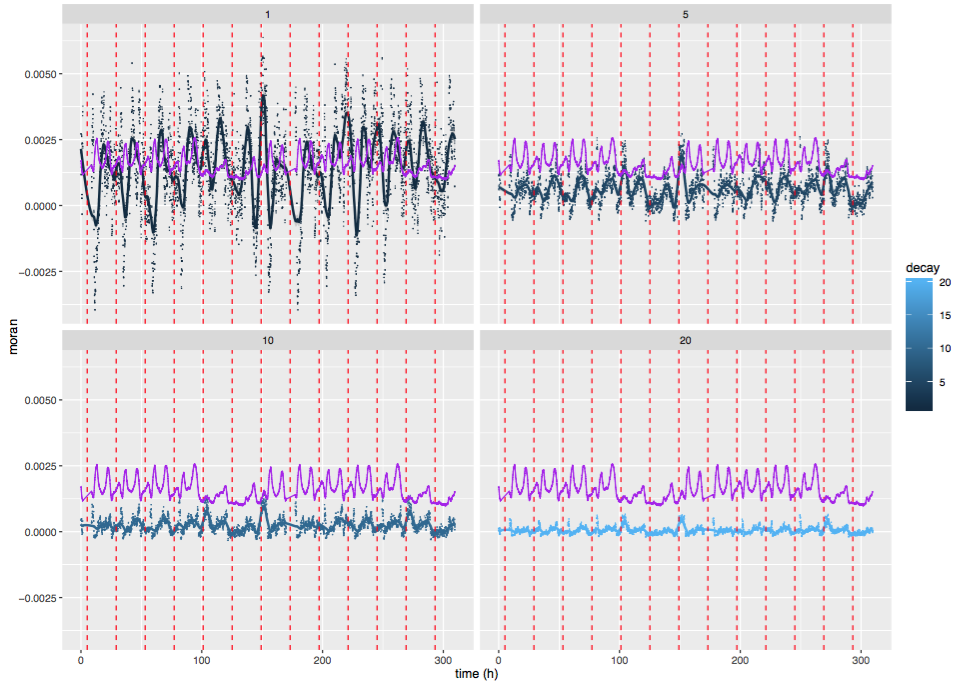
\includegraphics[width=\textwidth,height=0.8\textheight]{figures/moran_withCong}

}


%%%%%%%%%%%%%%%%%
\section{Discussion}
%%%%%%%%%%%%%%%%%


\sframe{Theoretical and Practical Implications}{

\justify

\textbf{Theoretical Implications}

\medskip

$\rightarrow$ Need for more systematic comparison of framework validity

(\cite{kryvobokov2013comparison} compares two LUTI models e.g.)

\medskip

$\rightarrow$ Can still be used e.g. for integration within more complex models

\bigskip
\bigskip

\textbf{Practical Implications}

\medskip

$\rightarrow$ Difficulty of transferring academic results to real-world engineering, that can be tied to habits, myths, political interests, etc.~\cite{commenges2013invention} ; \cite{offner1993effets}


}



%\sframe{Explanative Interpretations}{

% - not really interesting -

%}


\sframe{Possible Developments}{

\justify

\textbf{1. Further assessment of chaotic nature of traffic flows}

\medskip

$\rightarrow$ Study of spatio-temporal properties of Liapounov exponents

\cite{goldhirsch1987stability}, recently used in transportation research

\cite{tordeux2016jam}

\medskip

$\rightarrow$ Additional features for spatio-temporal data exploration : Kernel smoothing for wave visualization, localized plots, etc.


\bigskip

\textbf{2. Systematization of empirical assessment ; generic benchmarks for frameworks/model}

\medskip

$\rightarrow$ Similar use of a web-application for users to crowd-source their model/data as e.g. \cite{2016arXiv160606162C}


}



\sframe{Conclusion}{

$\rightarrow$ Simple but necessary empirical insights into SUE spatio-temporal stationarity

\medskip

$\rightarrow$ Construction of an open dataset : need for more openness, transparency, reproducibility

\medskip

$\rightarrow$ Strong need for more integrated research : theoretical-empirical, between disciplines, between approaches and objectives, between models (multi-modeling)


\bigskip
\bigskip
\bigskip


\footnotesize{ - All code available at \texttt{https://github.com/JusteRaimbault/TransportationEquilibrium}

\medskip

 - Paper preprint available at \texttt{http://arxiv.org/abs/1608.05266}
}

}






%%%%%%%%%%%%%%%%%%%%%
\begin{frame}[allowframebreaks]
\frametitle{References}
\bibliographystyle{apalike}
\bibliography{/Users/Juste/Documents/ComplexSystems/CityNetwork/Biblio/Bibtex/CityNetwork,biblio}
\end{frame}
%%%%%%%%%%%%%%%%%%%%%%%%%%%%












\end{document}







